\documentclass{standalone}

\usepackage[euler-digits]{eulervm}

\usepackage{tikz}
\usetikzlibrary{shapes}
\tikzset{every node/.style={draw,minimum size=2mm,inner sep=0pt}}
\tikzset{r/.style = {rectangle,fill=red!80!yellow}}
\tikzset{m/.style = {circle,fill=green}}
\tikzset{e/.style = {star,star points=5,fill=blue!60}}

\begin{document}
    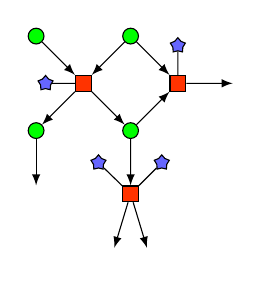
\begin{tikzpicture}[scale=1.2]
      \node[m] (1) at (0,2) {};
      \node[m] (2) at (0,1) {};
      \node[m] (3) at (1,2) {};
      \node[m] (4) at (1,1) {};
      \node[r] (5) at (0.5,1.5) {};
      \node[r] (6) at (1.5,1.5) {};
      \node[r] (7) at (1,0.33) {};
      \node[draw=none] (8) at (0.8,-0.33) {};
      \node[draw=none] (9) at (1.2,-0.33) {};
      \node[draw=none] (10) at (2.17,1.5) {};
      \node[draw=none] (11) at (0,0.33) {};

      \node[e] (e1) at (0.1,1.5) {};
      \node[e] (e2) at (1.5,1.9) {};
      \node[e] (e3) at (0.66,0.66) {};
      \node[e] (e4) at (1.33,0.66) {};

 \foreach \a/\b in {5/2,5/4,1/5,3/5,3/6,4/6,4/7,2/11,7/8,7/9,6/10}
   \draw[->,>=latex] (\a) -- (\b);

 \foreach \a/\b in {e1/5,e2/6,e3/7,e4/7}
   \draw (\a) -- (\b);


    \end{tikzpicture}
\end{document}
